\documentclass{article}

\usepackage[margin = 1in]{geometry}

\usepackage{amsmath, graphicx}
\graphicspath{ {./images/} }

\title{Ch. 16 Solutions}
\author{Principles of Microeconomics}
\date{\today}

\begin{document}

\maketitle

\section*{Quick Quiz}

\begin{enumerate}

\item (c) -- Without patents and copyright laws, firms and creators have less of an incentive to do research, invent new products, and create better art. Granting firms and creators temporary monopoly power has the potential to incentivize a more socially optimal amount of those activities.

\item (d) -- If a firm exhibits decreasing average total cost over the range of relevant output, then it can produce all of the output 
for the market more cheaply than multiple firms could. As a result, other firms are unlikely to compete. 

\item (b) -- Marginal revenue equals marginal cost because monopolies are profit-maximizers, and the quantity where marginal revenue equals marginal cost maximizes profit. 

Marginal revenue is less than price because of the price effect. When a monopoly increases its quantity supplied, it has to drop the market price in order to sell more units. As a result, the marginal revenue from selling an additional unit is the price of that unit minus the decrease in revenue from receiving a lower price on all the units it was already selling. 

\item (d) -- If a monopoly's fixed costs increase, its marginal cost remains the same. That means it still has the same profit-maximizing quantity, so it will still charge the price corresponding to that quantity on the demand curve.

Since the monopoly still produces the same quantity and sells it at the same price, its total revenue remains constant. Its total cost increase because of the increase in fixed costs. Profit equals total revenue minus total cost, so profit decreases. 

\end{enumerate}

\section*{Questions for Review}

\begin{enumerate}

\item Any pharmaceutical that has a patent is a government-created monopoly. On the one hand, the policy leads to higher prices for pharmaceuticals. On the other hand, it allows pharmaceutical companies to profit off of their research which incentivizes them to keep innovating better drugs. That's to say, the policy has its pros and cons.

\item A natural monopoly is an industry in which one firm can produce the market quantity more cheaply than multiple firms could. In other words, it's an industry with decreasing average total cost over the range of feasible market quantities. The size of the market is important because the larger the market, the more likely it is for average total cost to increase. If average total cost increases, it might become profitable for additional firms to enter and make the market more competitive.

\item For a monopoly, marginal revenue is less than the price of its good because of the price effect. When a monopoly increases its production by a unit, total revenue ($P \cdot Q$) is pulled in opposite directions. On the one hand, quantity increases which pulls total revenue up. That's the output effect. On the other hand, the price of the good must decrease in order to sell an additional unit which pulls total revenue down. That's the price effect. Altogether, that means a monopoly's marginal revenue is the price of the additional unit it sells minus the decrease in revenue from dropping the price on all of the units it was already selling. If the price effect is greater than the output effect, a monopoly's marginal revenue can certainly be negative. 

\item \phantom{x}
	\begin{center}
	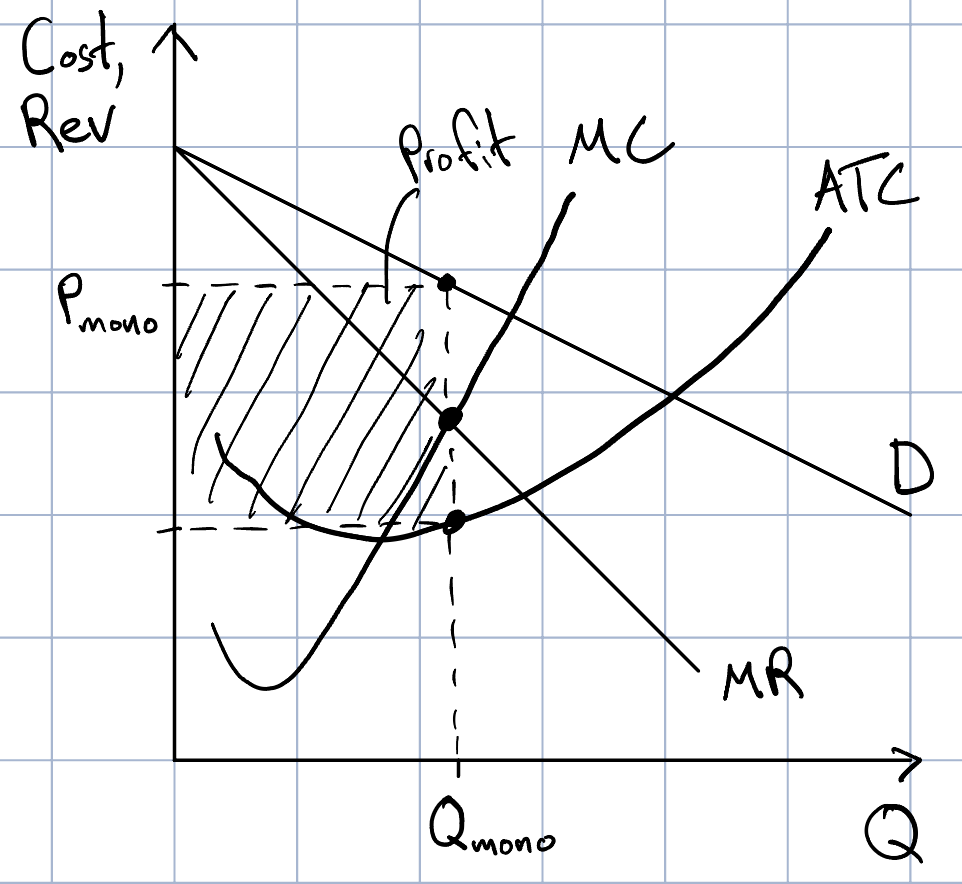
\includegraphics[width = 0.3\textwidth]{ch16_qfr4}
	\end{center}
	
\end{enumerate}

\end{document}